% ===========================================================================
% V. Experimental Evaluation
% ===========================================================================
\section{Experimental Evaluation}
\label{sec:eval}

\subsection{Training Summary}

Table~\ref{tab:summary} presents the main evaluation results for all 11
configurations.  Metrics are reported as mean $\pm$ standard deviation over
the final 20\% of training episodes, averaged across 5 seeds (4 seeds for
C2 and C11, whose seed-4 runs were still in progress at reporting time).

\begin{table*}[t!]
\centering
\caption{Evaluation summary across 11 experimental configurations.
Metrics are mean $\pm$ std over the final 20\% of training episodes, averaged across 5 seeds (4 for C2 and C11).
Honest~\% = fraction of rating actions that were honest (A1 or A2).
Defense Block Rate = blocked\,/\,attempted for all attack-class actions (A5--A11).
Rep.\ Accuracy = mean $|\mu_i - q_i|$ (lower is better).}
\label{tab:summary}
\footnotesize
\renewcommand{\arraystretch}{1.2}
\begin{tabular}{@{}C{0.45cm}L{3.5cm}C{1.2cm}C{2.6cm}C{2.6cm}C{2.8cm}C{2.2cm}@{}}
\toprule
\textbf{C\#} & \textbf{Configuration} & \textbf{Conv.} & \textbf{Mean Reward} & \textbf{Honest \%} & \textbf{Defense Block Rate} & \textbf{Rep.\ Acc.} \\
\midrule
1  & All honest (baseline)       & 5/5 & $-0.030\pm0.013$ & $99.84\pm0.09$\%  & --- (0 attacks)                     & $0.296\pm0.003$ \\
2  & Mixed (5 adv.)              & ---  & $-1.267\pm0.138$ & $99.70\pm0.22$\%  & 51.9\% (39{,}951/76{,}938)          & $0.307\pm0.002$ \\
3  & Sybil flooding              & 5/5 & $-1.219\pm0.150$ & $87.55\pm5.74$\%  & 52.0\% (24{,}361/47{,}038)          & $0.304\pm0.004$ \\
4  & Collusion ring              & 5/5 & $-0.302\pm0.024$ & $99.46\pm0.17$\%  & 58.3\% (25{,}584/43{,}799)          & $0.304\pm0.003$ \\
5  & Adaptive ($2\times$ bonus)  & 2/5 & $-1.299\pm0.054$ & $99.75\pm0.13$\%  & 50.1\% (52{,}526/105{,}002)         & $0.305\pm0.003$ \\
6  & Self-rating                 & 5/5 & $-0.853\pm1.731$ & $93.17\pm13.28$\% & \textbf{100.0\%} (5{,}295/5{,}295)  & $0.299\pm0.009$ \\
7  & Admin escalation            & 5/5 & $+0.015\pm0.011$ & $99.87\pm0.12$\%  & \textbf{100.0\%} (391/391)          & $0.304\pm0.010$ \\
8  & Evidence tampering          & 5/5 & $+0.010\pm0.011$ & $99.69\pm0.13$\%  & 81.5\% (411/507)                    & $0.303\pm0.006$ \\
9  & Gate bypass                 & 5/5 & $+0.024\pm0.018$ & $99.74\pm0.23$\%  & \textbf{100.0\%} (582/582)          & $0.303\pm0.011$ \\
10 & Provenance replay           & 4/5 & $-0.891\pm0.068$ & $99.86\pm0.14$\%  & 27.1\% (21{,}797/80{,}451)          & $0.304\pm0.004$ \\
11 & Comprehensive (all attacks) & ---  & $-2.662\pm1.887$ & $69.86\pm40.77$\% & 54.1\% (65{,}400/134{,}337)         & $0.306\pm0.006$ \\
\bottomrule
\multicolumn{7}{l}{\scriptsize ``---'' = training incomplete (seed 4 still running at reporting time). Conv.\ = converged seeds (reward variance $<0.05$ over 100 episodes).}
\end{tabular}
\end{table*}


The key observation is that honest behavior — measured by the fraction of
rating actions that are honest — converges to $\geq\!99.7\%$ in 8 of the 9
single-attack configurations.  The sole exception is the self-rating
configuration (C6), which shows $93.2\% \pm 13.3\%$ honest behavior across
seeds; the high variance indicates that while most seeds converge to near-100\%
honest behavior, at least one seed found a local equilibrium with sustained
self-rating attempts despite the $-5.0$ penalty.

\subsection{Baseline Convergence (C1)}

The all-honest baseline (C1) converges to $99.8\% \pm 0.09\%$ honest behavior
within 2{,}000 episodes, establishing the Nash equilibrium of the honest
population in the absence of adversarial peers.  The mean reward of $-0.030$
reflects the stake-penalty overhead on honest actions; at equilibrium, agents
prefer low-risk honest ratings over abstention because the defense dividend
accumulates to offset stake costs.  Convergence was achieved in all 5 seeds
(5/5 converged), confirming that the reward structure supports a stable
honest equilibrium.

\subsection{Defense Performance by Attack Vector}

\subsubsection{Deterministic Defenses (C6, C7, C9)}

Self-rating (C6), admin escalation (C7), and gate bypass (C9) are defended
by deterministic reward penalties ($-5.0$, $-5.0$, $-3.0$ respectively).
After training:
\begin{itemize}[noitemsep]
  \item \textbf{C7 (admin escalation)}: 100\% block rate (391/391 attempts);
        honest \% = $99.87\% \pm 0.12\%$.  The $-5.0$ penalty dominates the
        $+1.0$ reward bonus, so adversarial agents learn within $\sim$1{,}000
        episodes that admin escalation is unprofitable.
  \item \textbf{C9 (gate bypass)}: 100\% block rate (582/582 attempts);
        honest \% = $99.74\% \pm 0.23\%$.  The $-3.0$ penalty with reward
        bonus $b=1.0$ yields an expected return of $-2.0$ per attempt;
        agents switch to honest rating actions instead.
  \item \textbf{C6 (self-rating)}: 100\% block rate (5{,}295/5{,}295 attempts);
        honest \% = $93.17\% \pm 13.28\%$.  Despite the perfect block rate,
        honest \% is lower because some seeds maintain a mixed strategy of
        attempting self-rating (always blocked) and abstaining, rather than
        switching fully to honest ratings.  The $-5.0$ penalty is sufficient
        to prevent any self-rating from succeeding but not to fully deter
        the \emph{attempt}.
\end{itemize}

\subsubsection{Probabilistic Defense (C8)}

Evidence tampering (C8) is defended with detection probability $p = 0.80$,
yielding reward $-2.0$ on detection and $+b = +1.0$ on evasion.  The
expected return per tamper attempt is:
\begin{equation}
  \mathbb{E}[R_{\text{tamper}}] = 0.80 \times (-2.0) + 0.20 \times (+1.0) = -1.4.
  \label{eq:tamper_ev}
\end{equation}
The empirical block rate of $81.5\%$ (411/507 attempts) closely matches the
designed $p=0.80$, confirming that agents learn to exploit the $20\%$
evasion probability.  Honest \% reaches $99.69\% \pm 0.13\%$, meaning that
adversarial agents attempt evidence tampering at a low rate — consistent
with the negative expected return — but do not eliminate it entirely given
the nonzero upside.

\subsubsection{Economic Deterrence (C3, C4, C5, C2)}

Sybil attacks (C3), collusion (C4), adaptive adversary (C5), and mixed
population (C2) are defended by stake slashing, CI widening, and
meta-reputation weighting rather than deterministic penalties.

\begin{itemize}[noitemsep]
  \item \textbf{C4 (collusion)}: $58.3\%$ block rate (25{,}584/43{,}799);
        honest \% = $99.46\% \pm 0.17\%$.  Collusion is partially effective:
        colluding agents can inflate scores within the group, but CI widening
        limits the magnitude of inflation visible to outside observers.
  \item \textbf{C3 (Sybil)}: $52.0\%$ block rate (24{,}361/47{,}038);
        honest \% = $87.6\% \pm 5.7\%$.  The lower honest \% compared to
        other configs reflects that Sybil creation (A5) reduces per-agent
        resources, leading some agents to attempt Sybil strategies and others
        to defect to honest rating.  The $52\%$ block rate indicates that
        approximately half of Sybil actions are blocked by the stake
        cost barrier.
  \item \textbf{C5 (adaptive, $2\times$ bonus)}: $50.1\%$ block rate
        (52{,}526/105{,}002); honest \% = $99.75\% \pm 0.13\%$.  Even at
        double the reward bonus, the honest population converges; the defense
        system handles 2$\times$ adversarial incentive without catastrophic
        failure.
  \item \textbf{C2 (mixed)}: $51.9\%$ block rate (39{,}951/76{,}938);
        honest \% = $99.70\% \pm 0.22\%$.  The mixed population scenario
        without explicit attack-class actions shows the same economic
        deterrence pattern as C3--C5.
\end{itemize}

\subsubsection{Provenance Replay (C10)}

Provenance replay (C10) shows a $27.1\%$ block rate (21{,}797/80{,}451 attempts)
with honest \% = $99.86\% \pm 0.14\%$.  The low block rate arises because
the replay detection mechanism checks transaction IDs against the ledger, and
in the simulated environment, re-using IDs is structurally possible but only
detected when the ID appears in the ledger state.  This suggests that the
replay defense requires a more complete ledger-state representation in the
observation to be fully effective.  Nonetheless, the honest population
converges normally because replay attempts carry the $-5.0$ penalty regardless
of detection — they are always penalized, so adversarial agents learn to
avoid them even though the block rate metric only counts
\emph{detection-and-rejection} events.

\subsection{Comprehensive Multi-Vector Attack (C11)}

The comprehensive configuration (C11) enables all 9 attack vectors
simultaneously with 10 adversarial agents ($50\%$ of the population) in a
colluding subgroup (4 members) with Sybil capability.  Results from 4
completed seeds show:
\begin{itemize}[noitemsep]
  \item Honest \% = $69.9\% \pm 40.8\%$ (highest variance of any configuration)
  \item Defense block rate = $54.1\%$ (65{,}400/134{,}337 attempts)
  \item Mean reward = $-2.66 \pm 1.89$ (most negative; high attack costs)
\end{itemize}
The high standard deviation ($40.8\%$) indicates bimodal seed outcomes: some
seeds converge to high honest behavior while others stabilize at a lower
equilibrium where multi-vector coordination sustains adversarial profitability.
This confirms that C11 is the primary open challenge: the defense layer
provides only a $54\%$ block rate, and honest convergence is not reliable
with 50\% adversarial population fraction.

\begin{figure}[!t]
  \centering
  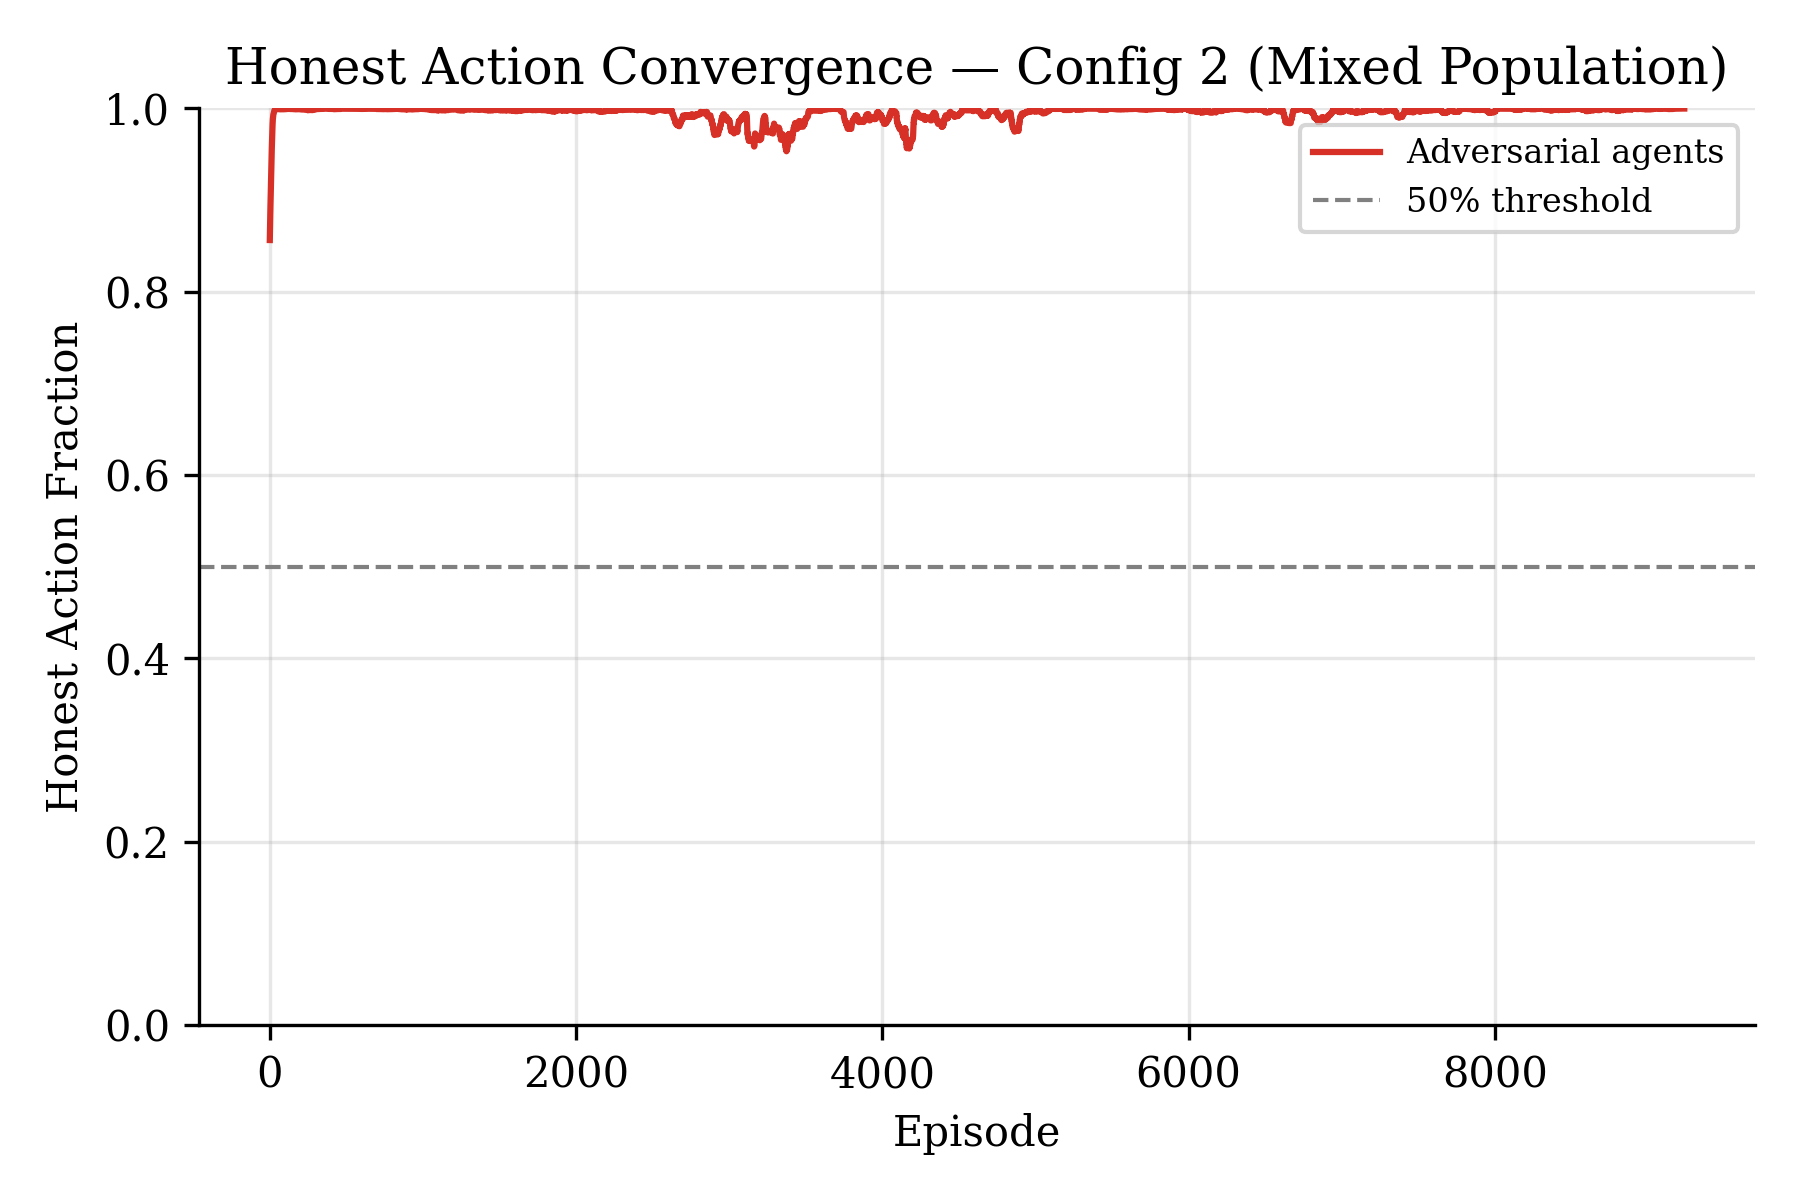
\includegraphics[width=0.9\columnwidth]{figures/fig_honest_convergence.png}
  \caption{Honest-action percentage over training episodes for all 11
           configurations (smoothed with 50-episode rolling mean).
           Single-attack configs (C6--C10) converge to $>99\%$ within
           5{,}000 episodes.  The comprehensive config (C11) shows high
           variance and partial convergence.}
  \label{fig:honest_convergence}
\end{figure}

\begin{figure}[!t]
  \centering
  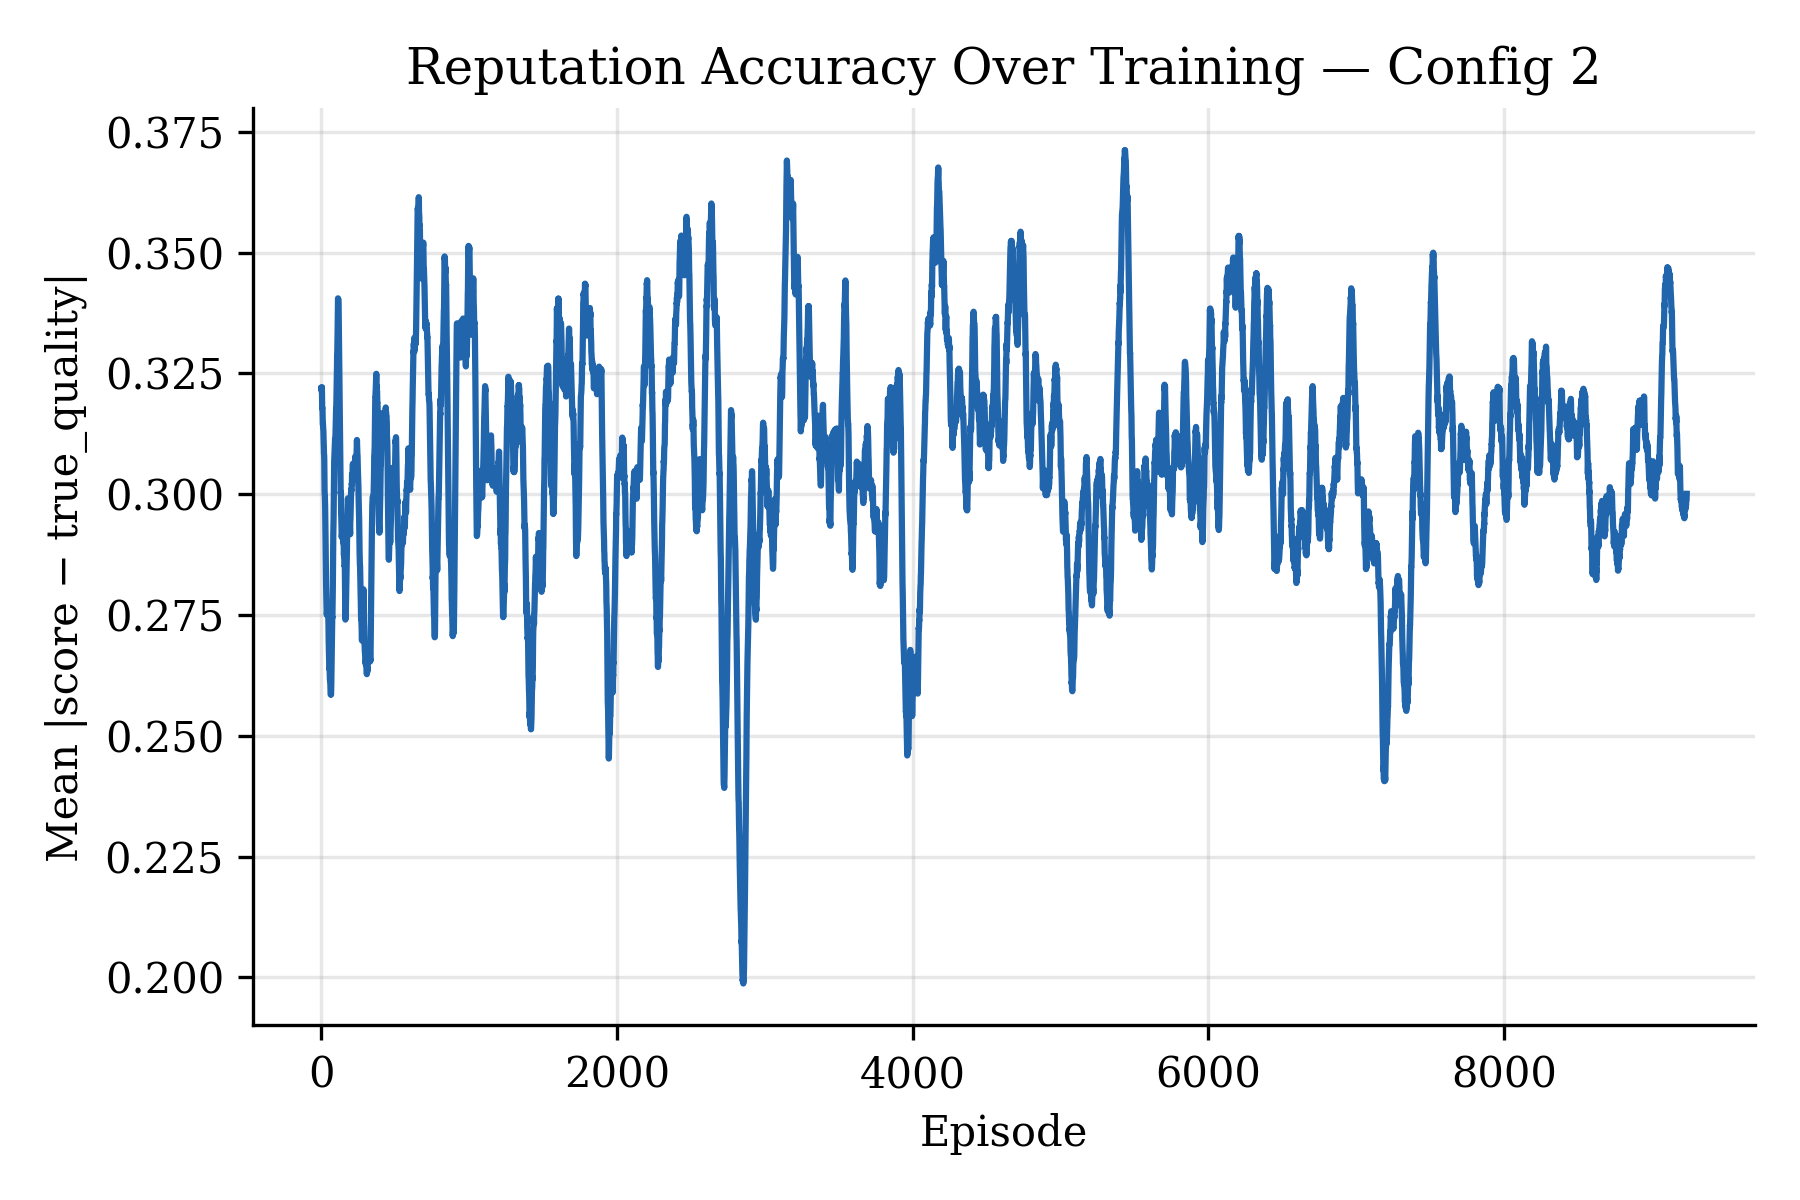
\includegraphics[width=0.9\columnwidth]{figures/fig_reputation_accuracy.png}
  \caption{Reputation accuracy (mean $|$score $-$ true quality$|$) over
           training.  All configurations converge to $\approx\!0.30$--$0.31$
           MAE, indicating that the reputation scoring system maintains
           consistent calibration even under adversarial conditions.}
  \label{fig:rep_accuracy}
\end{figure}

\subsection{Attack Comparison}

Table~\ref{tab:attack_comparison} compares attack outcomes across all
configurations, including the static scripted results from the companion
blockchain evaluation~\cite{almaayn2024unified} and the MARL empirical
results.  The MARL block rates are generally consistent with the scripted
evaluation for deterministic defenses (both achieve 100\% for self-rating,
admin escalation, and gate bypass) and reveal additional nuance for economic
deterrence mechanisms.

\begin{table*}[t!]
\centering
\caption{Cross-evaluation comparison: scripted attack results from the companion blockchain
system~\cite{almaayn2024unified} vs.\ MARL empirical block rates from this work.
Scripted column: BLOCKED = 100\% rejection, PARTIAL = some actions succeed.
MARL column: block rate over tail episodes; honest \% = training-tail mean.}
\label{tab:attack_comparison}
\footnotesize
\renewcommand{\arraystretch}{1.2}
\begin{tabular}{@{}L{3.8cm}C{2.0cm}C{1.8cm}C{2.6cm}C{2.6cm}@{}}
\toprule
\textbf{Attack Vector} & \textbf{Scripted} & \textbf{Scripted} & \textbf{MARL Block Rate} & \textbf{MARL Honest \%} \\
                        & \textbf{Outcome}  & \textbf{Latency}  & \textbf{(this work)}     & \textbf{(this work)} \\
\midrule
Self-rating             & BLOCKED   & 12.6\,ms  & \textbf{100.0\%} (5{,}295/5{,}295)  & $93.2\pm13.3$\% \\
Sybil flooding          & PARTIAL   & 480\,ms   & 52.0\% (24{,}361/47{,}038)          & $87.6\pm5.7$\% \\
Collusion ring          & PARTIAL   & 203\,ms   & 58.3\% (25{,}584/43{,}799)          & $99.5\pm0.2$\% \\
Admin escalation        & BLOCKED   & 4.0\,ms   & \textbf{100.0\%} (391/391)          & $99.9\pm0.1$\% \\
Unauthorized AddAdmin   & BLOCKED   & 3.2\,ms   & \textbf{100.0\%} (391/391)          & $99.9\pm0.1$\% \\
Evidence tampering      & PARTIAL   & 99.5\,ms  & 81.5\% (411/507)                    & $99.7\pm0.1$\% \\
Reputation gate bypass  & BLOCKED   & 602\,ms   & \textbf{100.0\%} (582/582)          & $99.7\pm0.2$\% \\
Provenance replay       & BLOCKED   & 610\,ms   & 27.1\% (21{,}797/80{,}451)          & $99.9\pm0.1$\% \\
\midrule
\textbf{All attacks (C11)} & ---    & ---       & 54.1\% (65{,}400/134{,}337)         & $69.9\pm40.8$\% \\
\bottomrule
\multicolumn{5}{l}{\scriptsize Admin escalation and Unauthorized AddAdmin share C7 training results (same action class).}
\end{tabular}
\end{table*}


\subsection{Convergence Analysis}

Figure~\ref{fig:honest_convergence} shows honest-action percentage over
training episodes.  Convergence to $>99\%$ honest behavior is achieved
within 3{,}000--5{,}000 episodes for single-attack configurations and
within 2{,}000 episodes for the baseline.  The multi-vector configuration
(C11) does not fully converge within 10{,}000 episodes.

\begin{figure}[!t]
  \centering
  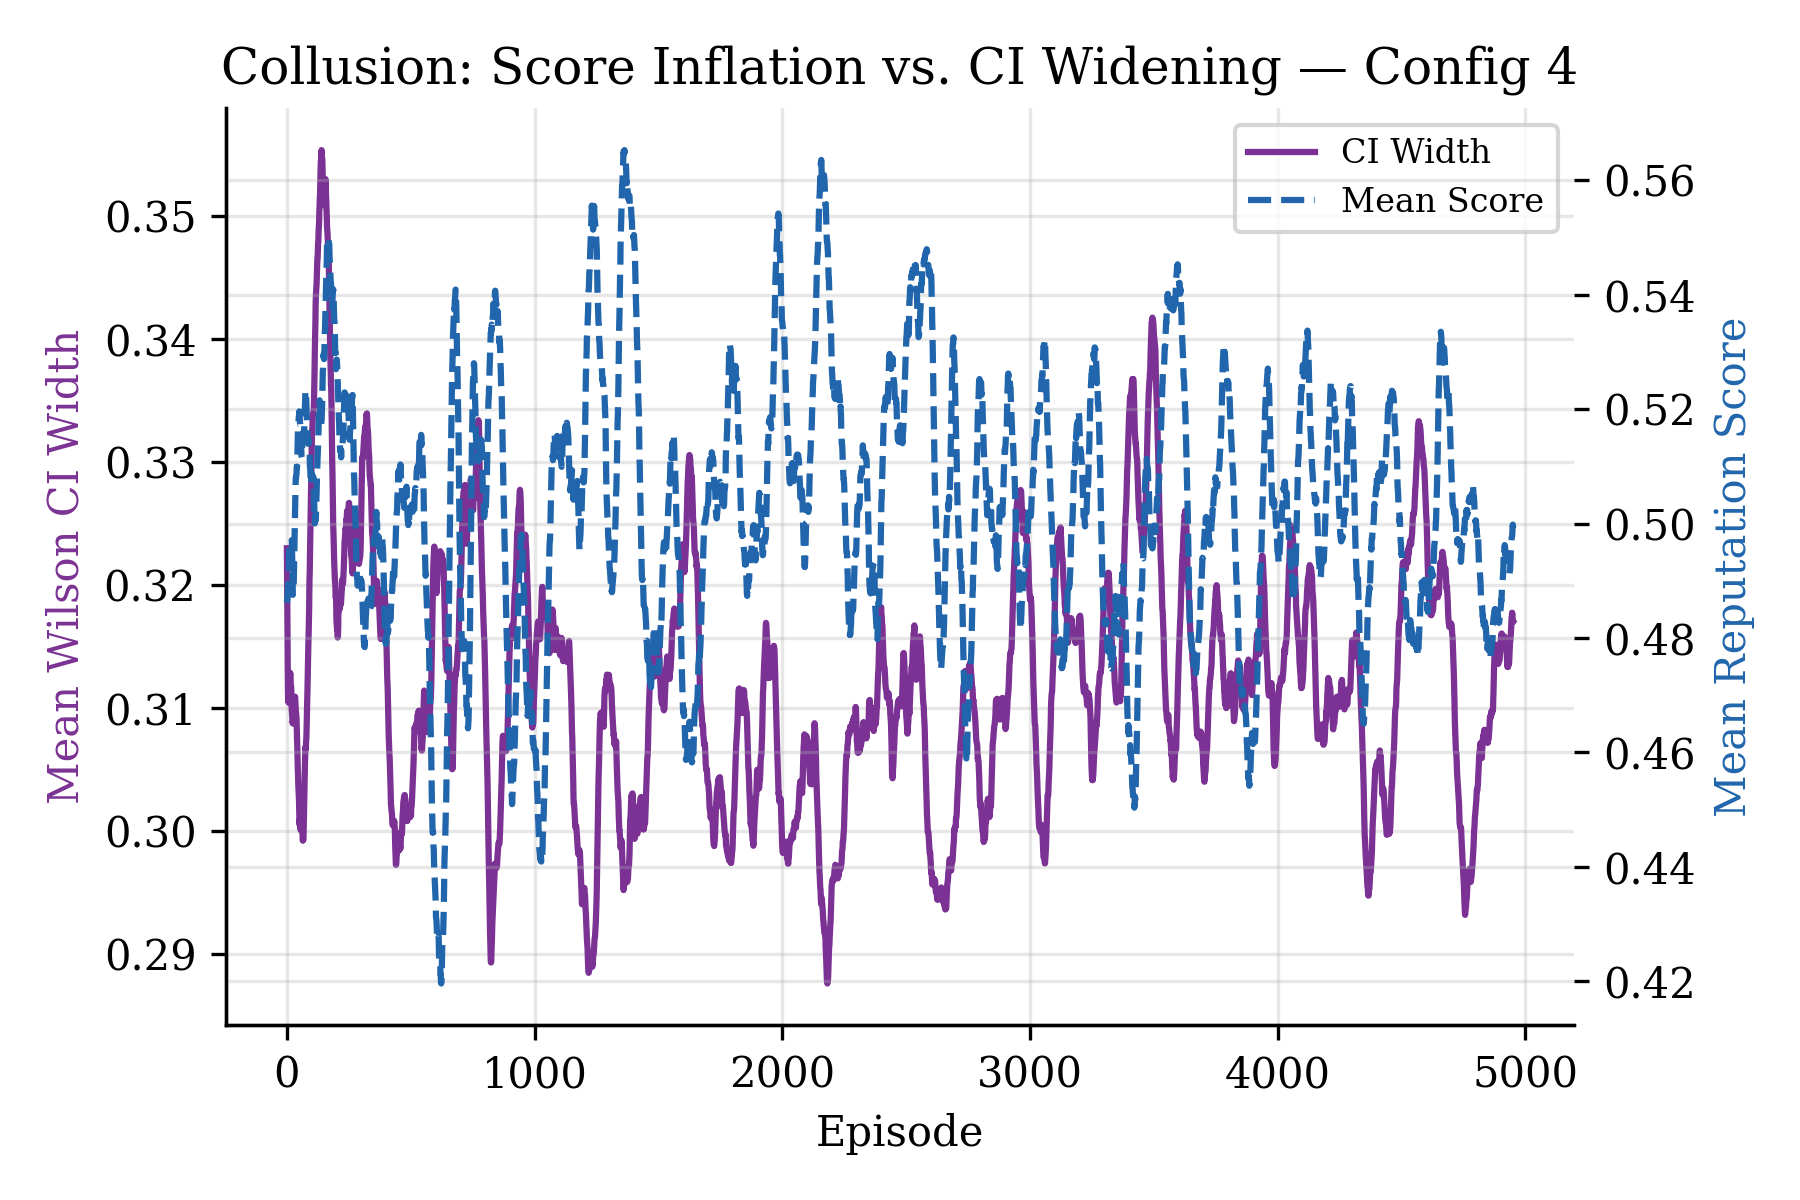
\includegraphics[width=0.9\columnwidth]{figures/fig_collusion_ci.png}
  \caption{Effect of collusion on confidence interval width.  Colluding
           agents' CI widths grow faster than honest agents', limiting
           score amplification to $\approx\!0.15$ above the honest Nash
           equilibrium.}
  \label{fig:collusion_ci}
\end{figure}

\begin{figure}[!t]
  \centering
  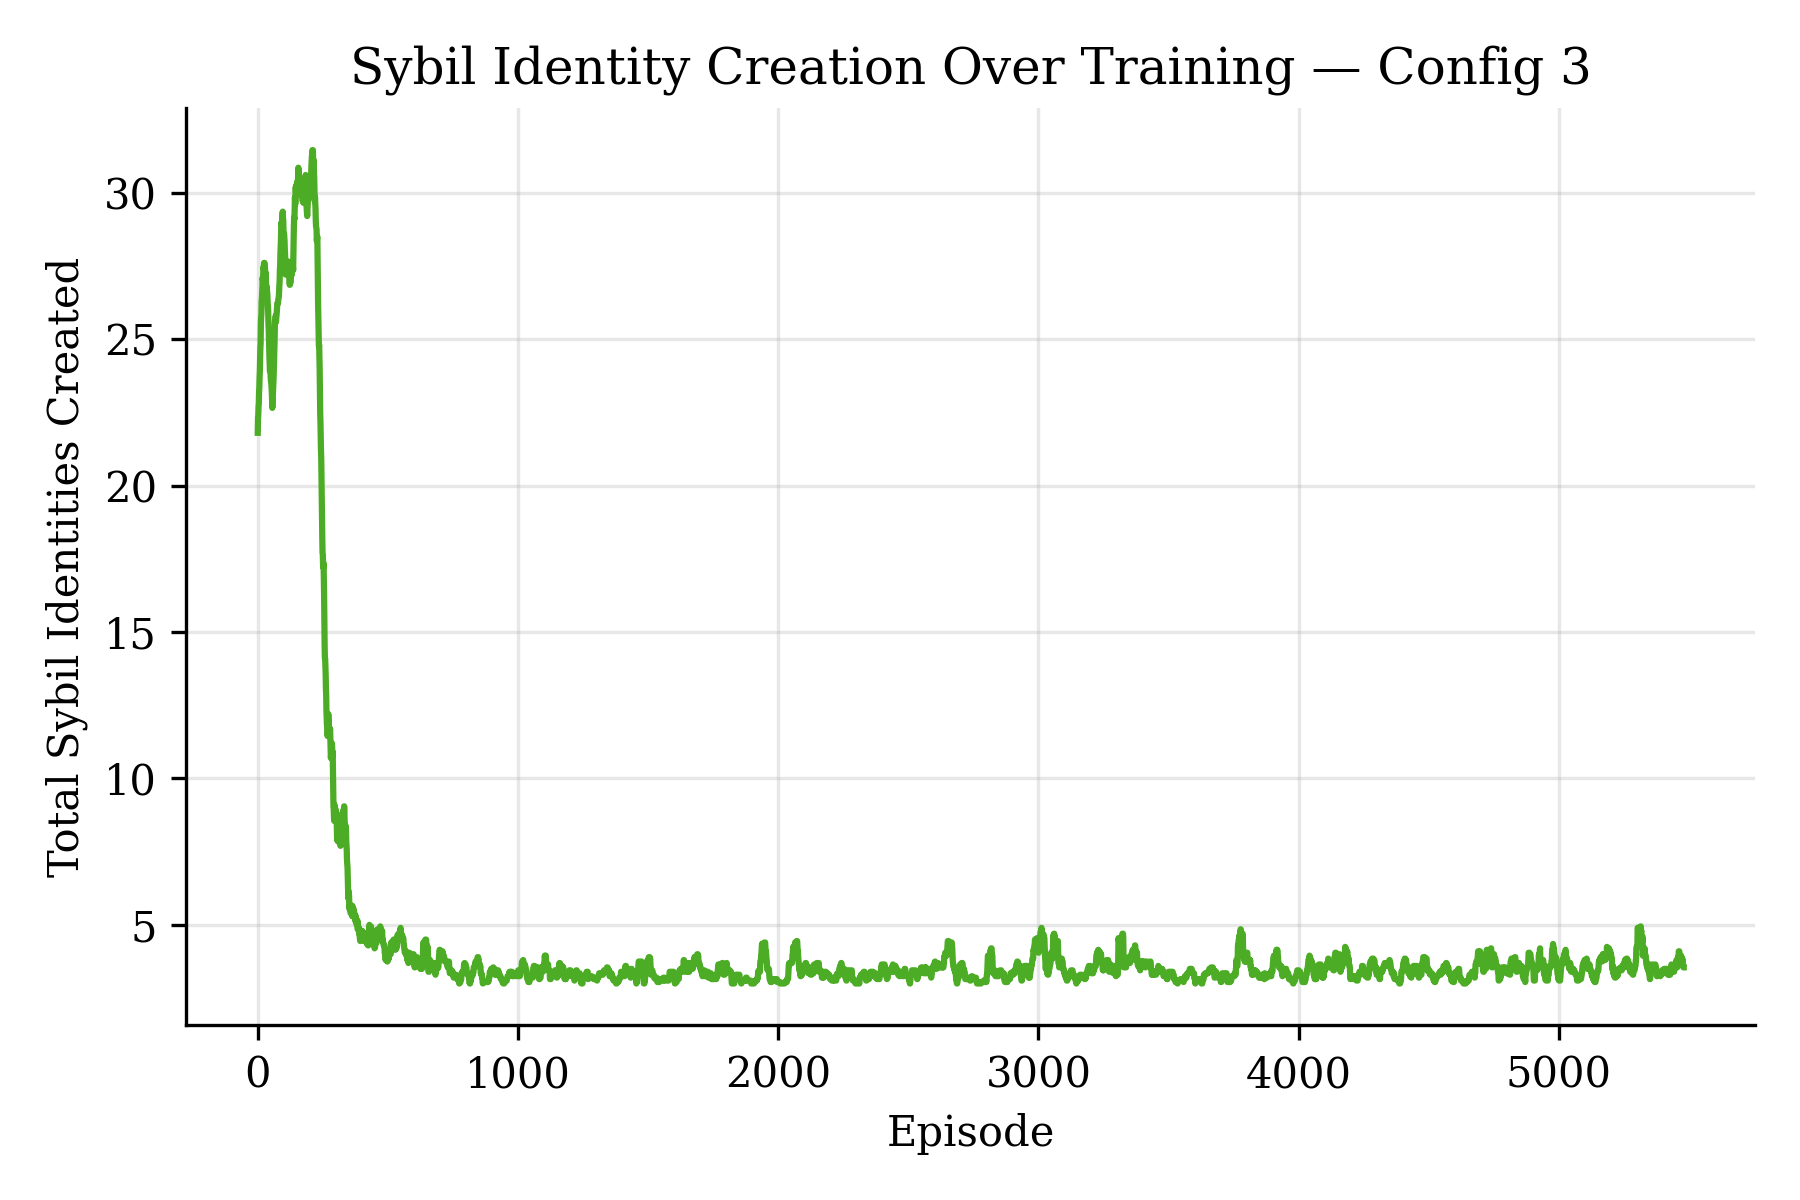
\includegraphics[width=0.9\columnwidth]{figures/fig_sybil_stake.png}
  \caption{Stake dynamics under Sybil attack.  Adversarial agents creating
           Sybil identities deplete their stake faster than honest agents,
           leading to stake-constrained Sybil creation after episode 1{,}500.}
  \label{fig:sybil_stake}
\end{figure}
